\subsection{Background Selection} % 删除了多余的空格
\label{sec:monoZ_bkg}

Three dedicated background control regions (CRs) are defined to determine normalization factors for the dominant backgrounds in the signal region (SR). The CR definitions are summarized below.

\paragraph{The $e\mu$ CR:}
This region is defined identically to the SR, except that the two leptons are required to have different flavours. It constrains the non-resonant backgrounds from $t\bar{t}$, single top-quark, $\text{WW}$, and $\text{Z} \to \tau\tau$ processes. The $e\mu$ CR is approximately 98\% pure in the non-resonant background.

\paragraph{The $3\ell$ CR:}
This region, requiring exactly three leptons, is used to normalize the $\text{WZ}$ background. A $\text{Z}$ boson candidate is formed from two opposite-charge, same-flavour leptons with $p_{\text{T}}^{\ell} > 20,\,30~\text{GeV}$ and invariant mass $76 < m_{\ell\ell} < 106~\text{GeV}$. An additional lepton with $p_{\text{T}}^{\ell} > 20~\text{GeV}$ is required. Events must satisfy $E_{\text{T}}^{\text{miss}} > 30~\text{GeV}$ and $S_{E_{\text{T}}^{\text{miss}}} > 3$. The transverse mass of the $\text{W}$ boson candidate is required to be
\begin{equation}
m_{\text{T}}^{\text{W}} =
\sqrt{
2\,p_{\text{T}}^{\ell}\,
E_{\text{T}}^{\text{miss}}\,
\left(1 - \cos\Delta\phi(\ell, E_{\text{T}}^{\text{miss}})\right)
}
> 60~\text{GeV},
\end{equation}
where $\Delta\phi(\ell, E_{\text{T}}^{\text{miss}})$ is the azimuthal angle between the third lepton and the missing transverse momentum. The $3\ell$ CR has a purity of about 93\% in $\text{WZ}$ events.

\paragraph{The $4\ell$ CR:}
This region, requiring exactly four leptons, constrains the $\text{ZZ}$ background. Events must contain two same-flavour, oppositely charged lepton pairs with $p_{\text{T}}^{\ell} > 7,\,15,\,15,\,27~\text{GeV}$ when ordered in increasing $p_{\text{T}}$. If all four leptons have the same flavour, the pairing that minimizes $|m_{\ell\ell_1} - m_{\text{Z}}| + |m_{\ell\ell_2} - m_{\text{Z}}|$ is chosen, where $m_{\text{Z}} = 91.19~\text{GeV}$. Both lepton pairs are required to satisfy $76 < m_{\ell\ell} < 106~\text{GeV}$.

To mimic the SR topology, one randomly chosen lepton pair is treated as invisible when calculating ${E_{\text{T}}^{\text{miss}}}'$ and $S_{{E_{\text{T}}^{\text{miss}}}'}$. The same selection criteria as in the SR are then applied:
${E_{\text{T}}^{\text{miss}}}' > 90~\text{GeV}$,
$S_{{E_{\text{T}}^{\text{miss}}}'} > 9$, and
$\Delta R_{\ell\ell} < 1.8$ for the remaining lepton pair. The $4\ell$ CR is nearly 100\% pure in $\text{ZZ}$ events.

The definitions of these control regions are summarized in Table~\ref{tab:SR_CR_selection}, columns~2--4.

\begin{table}[htbp]
\centering
\small
\begin{tabular}{c|c|c|c}
\hline
 SR & $e\mu$ CR & $3\ell$ CR & $4\ell$ CR \\
\hline
\multicolumn{4}{c}{Single lepton trigger matched to offline lepton} \\
\multicolumn{4}{c}{$b$-jet veto} \\
\hline
%\multicolumn{5}{c}{Vertex} \\
%\multicolumn{5}{c}{Event cleaning} \\

$\ell^+\ell^-$ pair & $e^\pm\mu^\mp$ pair & $\ell^+\ell^-$ pair + $\ell'$ & 2 pairs of $\ell^+\ell^-$ \\
\hline
$p_{\text{T}}^{\ell} > 20,\,30~\text{GeV}$ & $p_{\text{T}}^{\ell} > 20,\,30~\text{GeV}$ & $p_{\text{T}}^{\ell} > 20,\,30,\,20~\text{GeV}$ & $p_{\text{T}}^{\ell} > 7,\,15,\,15,\,27~\text{GeV}$ \\
\hline
$76 < m_{\ell\ell} < 106~\text{GeV}$& $76 < m_{e\mu} < 106~\text{GeV}$ & $76 < m_{\ell\ell} < 106~\text{GeV}$& $76 < m_{\ell\ell} < 106~\text{GeV}$ \\
\hline
\multicolumn{2}{c|} {$E_{\text{T}}^{\text{miss}} > 90~\text{GeV}$} &
$E_{\text{T}}^{\text{miss}} > 30~\text{GeV}$ & ${E_{\text{T}}^{\text{miss}}}' > 90~\text{GeV}$ \\
\hline
\multicolumn{2}{c|} {$\Delta R_{\ell\ell} < 1.8$} &
$m_{\text{T}}^{\text{W}} > 60~\text{GeV}$ & $\Delta R_{\ell\ell} < 1.8$ \\
\hline
\multicolumn{2}{c|}{$S_{E_{\text{T}}^{\text{miss}}} > 9$} 
& $S_{E_{\text{T}}^{\text{miss}}} > 3$ 
& $S_{{E_{\text{T}}^{\text{miss}}}'} > 9$ \\
\hline
\end{tabular}
\caption{\rm Event selection criteria for the signal region (SR) and control regions (CRs).}
\label{tab:SR_CR_selection}
\end{table}

%%%%%%%%%%%%%%%%%%%%%
The yields of signal and all backgrounds are estimated through simultaneous likelihood fits in the SR and CRs, using MC simulation as input. The dominant background in the SR is the $\text{ZZ}$ process, followed by $\text{WZ}$, $\text{Z}$+jets, and the non-resonant backgrounds ($\text{WW}$, $t\bar{t}$, single top-quark, and $\text{Z} \to \tau\tau$), which are treated together. Small contributions arise from $\text{VVV}$, $t\bar{t}\text{V}$, and $\text{ZZ} \to 4\ell$ processes.

%The $ZZ$ and non-resonant backgrounds have the same topology as the signal, consisting of two leptons and $E_{\mathrm{T}}^{\mathrm{miss}}$. The SM Higgs boson decay $H \to ZZ \to 4\nu$ is included as part of the signal, while other Higgs decay modes are estimated to be small and are neglected. The $WZ$ background enters the SR when one of the leptons is not reconstructed.

%In most $Z$+jets background events, significant $E_{\mathrm{T}}^{\mathrm{miss}}$ arises from mismeasurement of jet energies or from neutrinos or muons that are not reconstructed, typically originating from semileptonic heavy-flavor decays. The normalization of the MC prediction for $Z$+jets was cross-checked using events with low $E_{\mathrm{T}}^{\mathrm{miss}}$ significance, $S_{E_{\mathrm{T}}^{\mathrm{miss}}} < 9$, which has high purity for this process. 
%A sample of $\gamma$+jets events, which has production diagrams similar to those of $Z$+jets, was used to validate the MC description of the data shape. In both cases, the MC prediction and data were found to agree within statistical and systematic uncertainties.
%%%%%%%%%%%%%%%%%%%%%

\section{Improving the Signal Sensitivity with a BDT}

The sensitivity of the $\text{H} \to \text{invisible}$ search is enhanced using a boosted decision tree (BDT) implemented in the TMVA package~\cite{Hoecker:2007tmva} to improve the separation between signal and background events. The BDT combines multiple kinematic variables, chosen for their discriminative power, into a single output that achieves greater separation than any individual variable.

Eight input variables are used: $E_{\text{T}}^{\text{miss}}/H_{\text{T}}$, $S_{E_{\text{T}}^{\text{miss}}}$, $H_{\text{T}}$, $f_{\text{soft}} = |1 - |\vec{E}_{\text{T}}^{\text{miss}} + \vec{p}_{\text{T}}^{\text{jets}}| / p_{\text{T}}^{\ell\ell}|$, $m_{\ell\ell}$, $\Delta R_{\ell\ell}$, $Y_{\ell\ell}$ (rapidity of the dilepton system), and $\Delta\phi(\ell\ell, E_{\text{T}}^{\text{miss}})$ (azimuthal angle between the dilepton transverse momentum and $E_{\text{T}}^{\text{miss}}$). Additional variables were evaluated, but provided negligible improvement.

The BDT is trained in the signal region (SR) using simulated $\text{ZH} \to \ell\ell + \text{invisible}$ signal events and the combined background samples selected in the CRs. The resulting BDT output distribution, shown in Figure~\ref{fig:bdt}(a), is used as the input to the profile likelihood fit in the SR and the $e\mu$ CR, shown in Figure~\ref{fig:bdt}(b). In the $3\ell$ and $4\ell$ CRs, the $E_{\text{T}}^{\text{miss}}$ distribution is used instead, as several BDT input variables exhibit significantly different shapes between the CRs and SR.

\begin{figure}[htbp]
    \centering
\subfloat[]{
    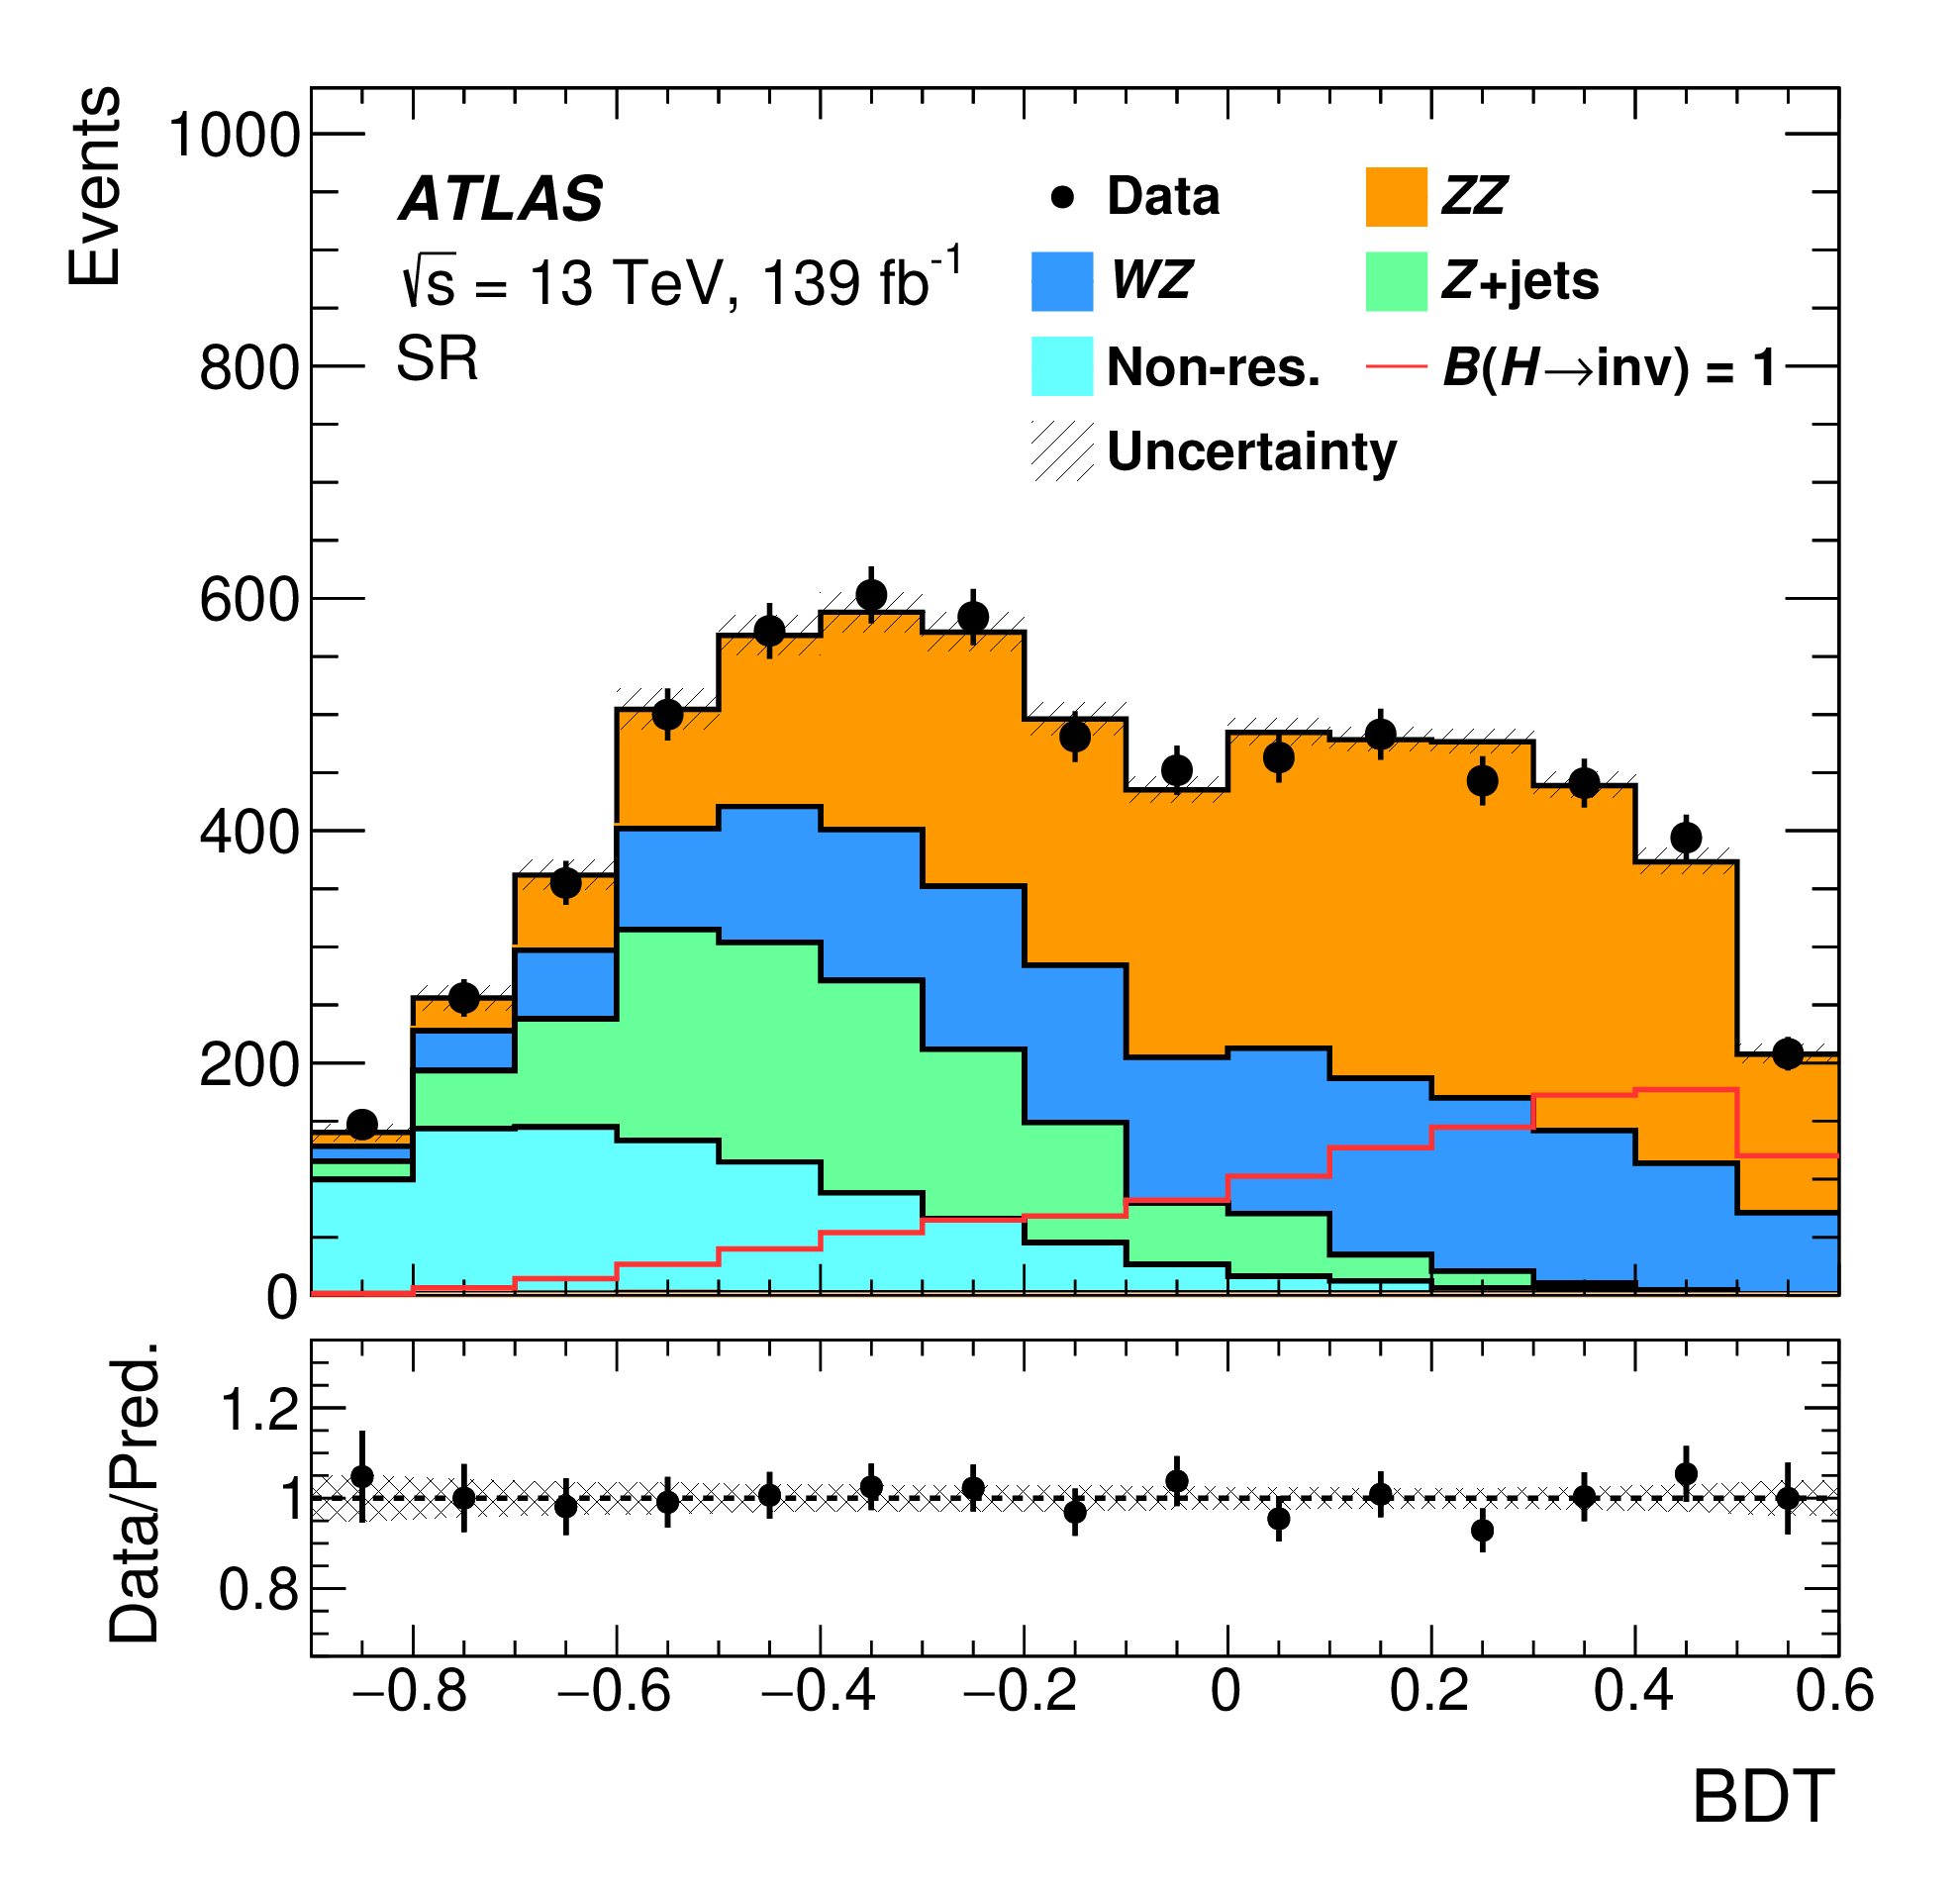
\includegraphics[width=0.48\linewidth]{figures/ch6-DM/fig_03a.png}}
\subfloat[]{    
    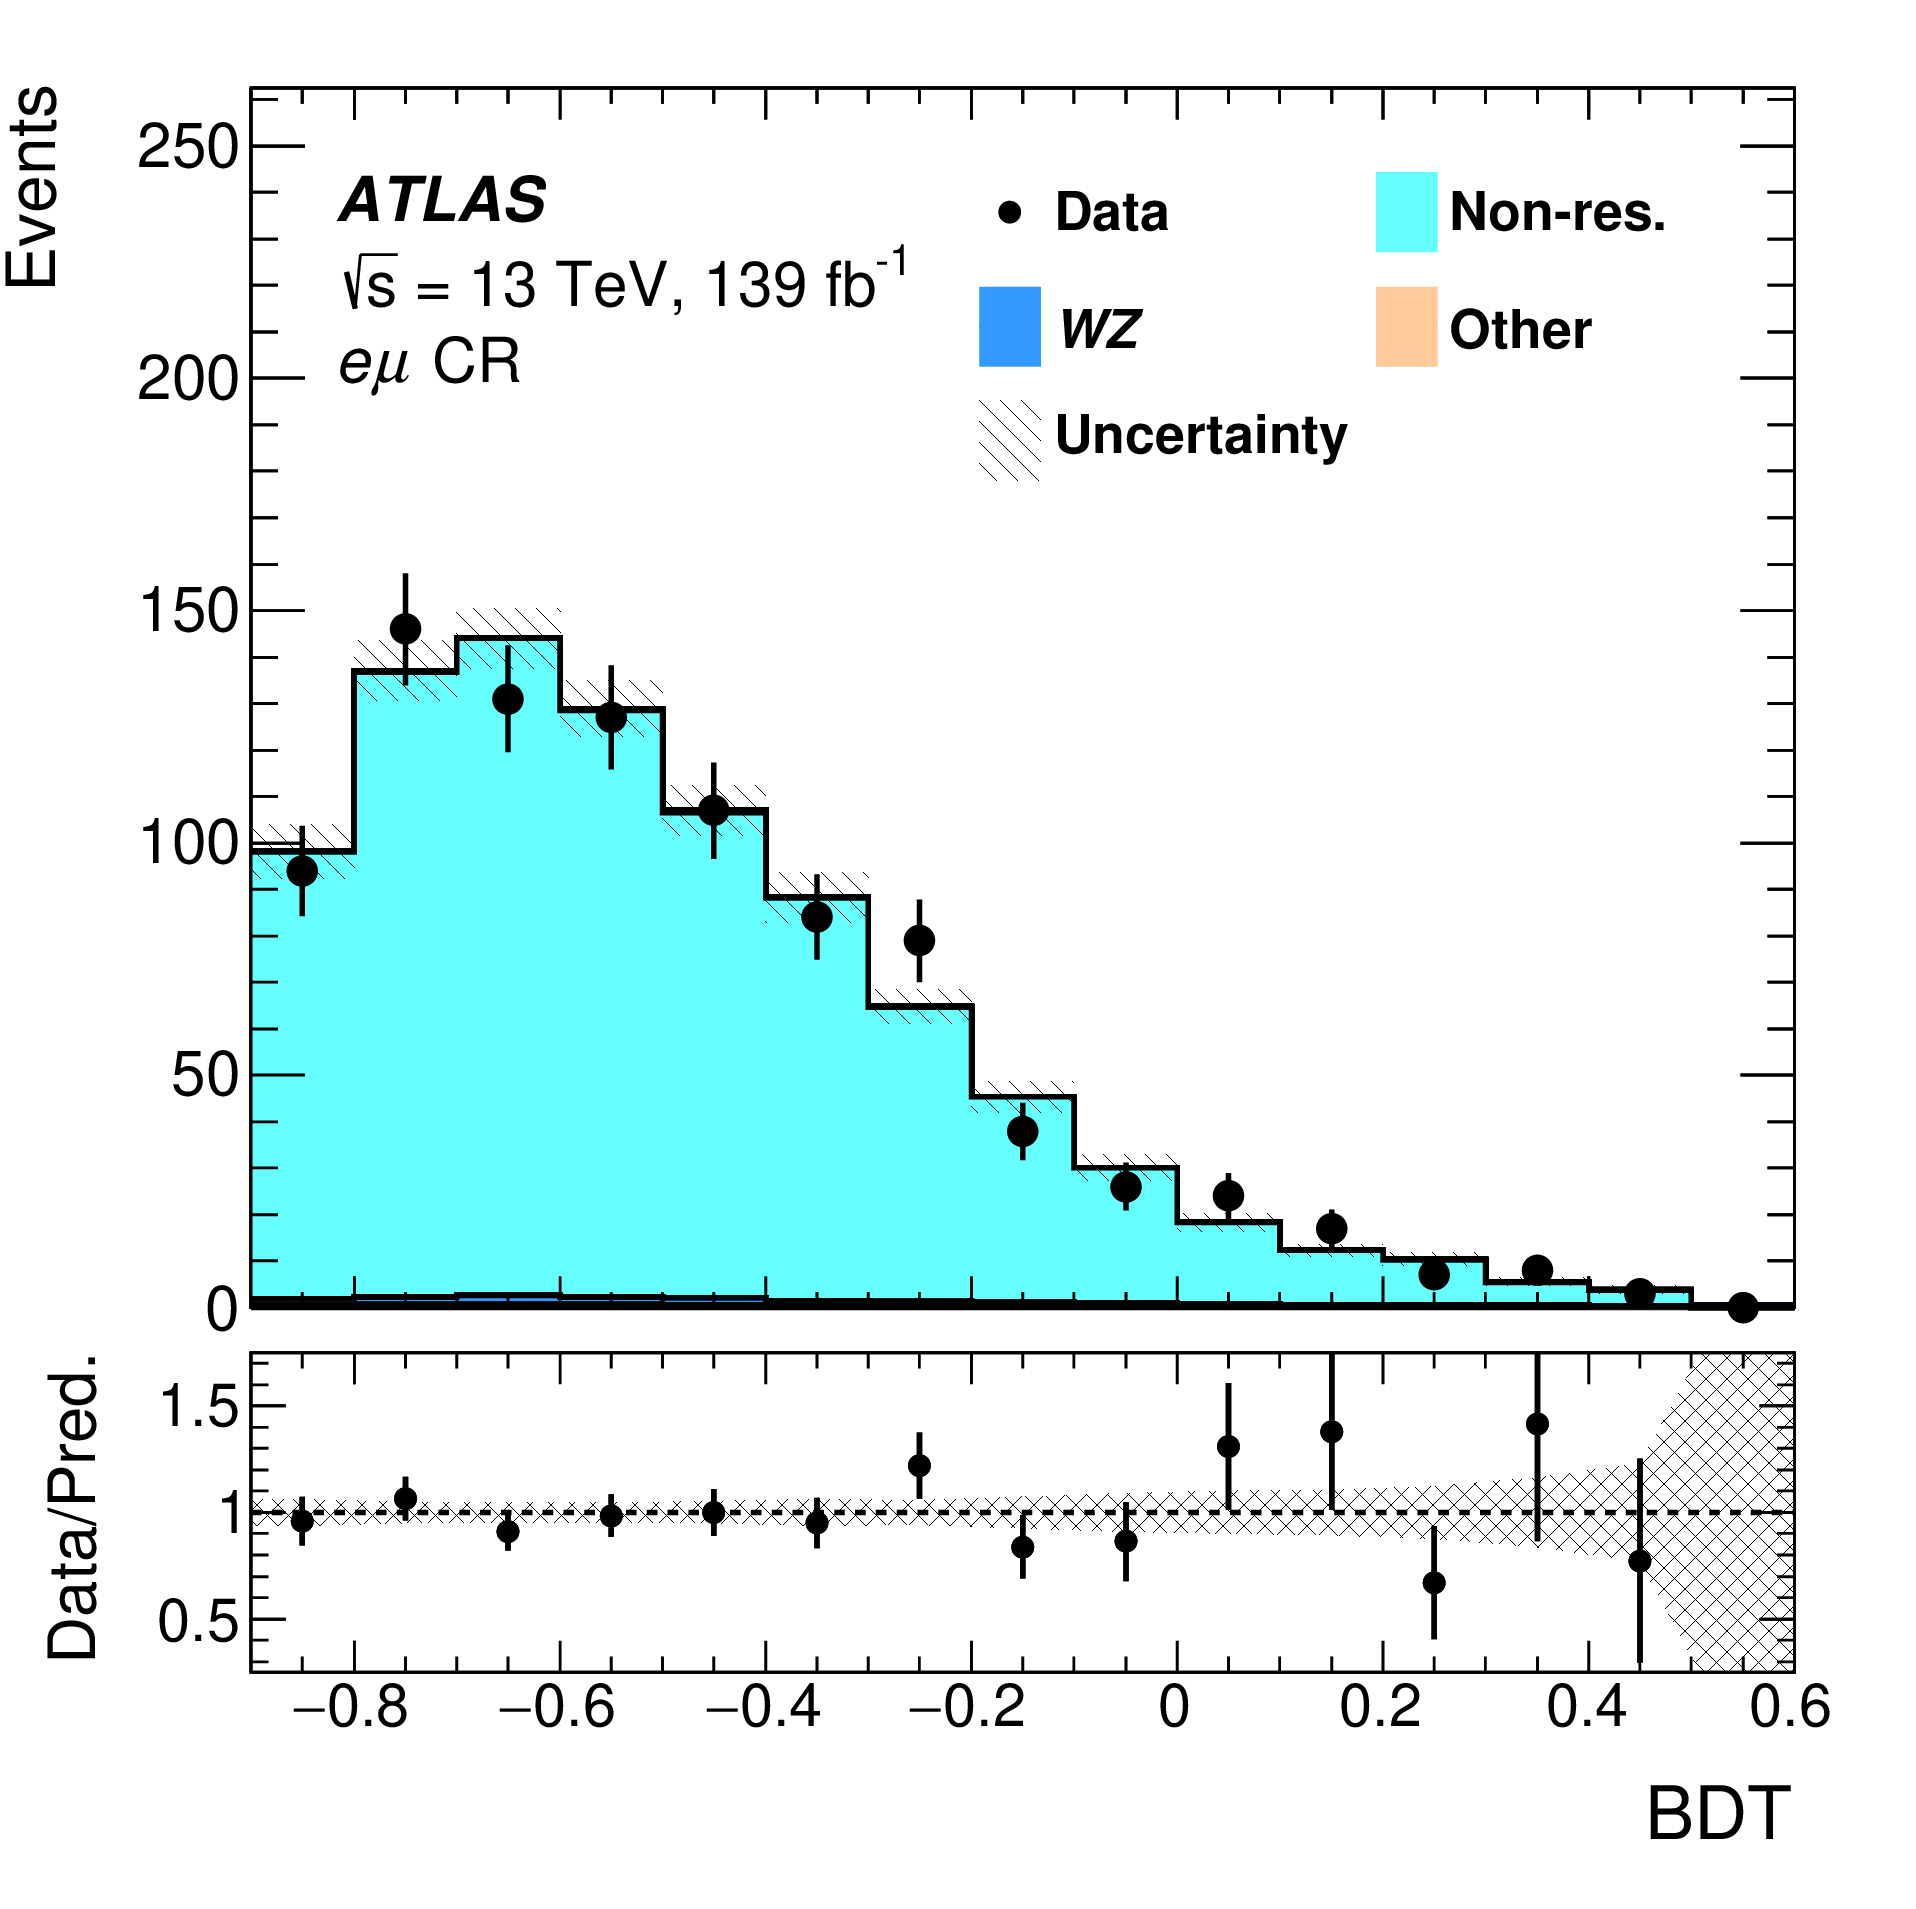
\includegraphics[width=0.47\linewidth]{figures/ch6-DM/fig_02c.png}}    
    \caption{Data and MC comparison of BDT output distributions. (a) signal and background spectra in the SR, and (b) the non-resonant $e\mu$ CR BDT spectrum.}
    \label{fig:bdt}
\end{figure}
    

\section{Data and MC Comparison in SR and CRs}

Table~\ref{tab:event-yields} gives the summary of signal and control region yields after the simultaneous fit for the $\text{ZH}(\to \text{inv.})$ signal. Also given is the total post-fit uncertainty of each number.

Figure~\ref{fig:SR-CR-plot} shows data and MC prediction (after fit) comparison in distributions: (a) $m_{\text{T}}^{\text{ZZ}}$ in SR, (b) $E_{\text{T}}^{\text{miss}}$ in $3\ell$ CR, (c) $E_{\text{T}}^{\text{miss}}$ in $4\ell$ CR, and (d) $m_{\text{T}}^{\text{ZZ}}$ in $e\mu$ CR. In general, MC predictions agree with data in both SR and all three CRs.

\begin{table}[htbp]
    \centering
\renewcommand{\arraystretch}{1.25}    
    \begin{tabular}{lcccc}
\hline    \hline
         &  SR  & $e\mu$ CR & 3$\ell$ CR & 4$\ell$ CR \\
\hline         
Data     &  6382    &    891      &   11622  &  314   \\
\hline
Expected yields (post-fit) & $6385 \pm 81$ & $895 \pm 29$ & $11620 \pm 110$& $296 \pm 11$ \\    
\hline         
$\text{ZH} \to \ell\ell + \text{inv.}$    & $4 \pm 110$  &  -   &  -      & -            \\
$\text{ZH} \to \ell\ell\nu\nu$ & $2681 \pm 110$ & $0.763 \pm 0.064$ &$2.61 \pm 0.018$ & - \\
$\text{WZ}$         &  $1595 \pm 34$ &$11.6 \pm 1.1$  &$10623 \pm 150$  & -  \\
$\text{Z}$+jets     & $1111 \pm 100$ &$0.79 \pm 0.30$  &$235 \pm 89$  & - \\         
Non-resonant        & $881 \pm 39$ & $876 \pm 29$ &$220 \pm 31$  & -  \\
$\text{ZZ} \to 4\ell$& $85.8 \pm 5.5$ & $0.621 \pm 0.056$ &$443 \pm 40$  & $295 \pm 11$  \\
$t\bar{t}\text{V}$ & $12.7 \pm 2.8$ & $1.76 \pm 0.41$ & $53 \pm 12$ &  - \\
$\text{VVV}$       & $13.0 \pm 6.2$ & $3.1 \pm 1.4$ & $44 \pm 20$ &  $0.48 \pm 0.23$\\       \hline\hline 
    \end{tabular}         
    \caption{\rm Summary of SR and CR yields after the simultaneous fit for the $\text{ZH}(\to \text{inv.})$ signal. Also given is the total post-fit uncertainty of each number.}
    \label{tab:event-yields}
\end{table}

\begin{figure}[!htbp]
    \centering
    \subfloat[]{
    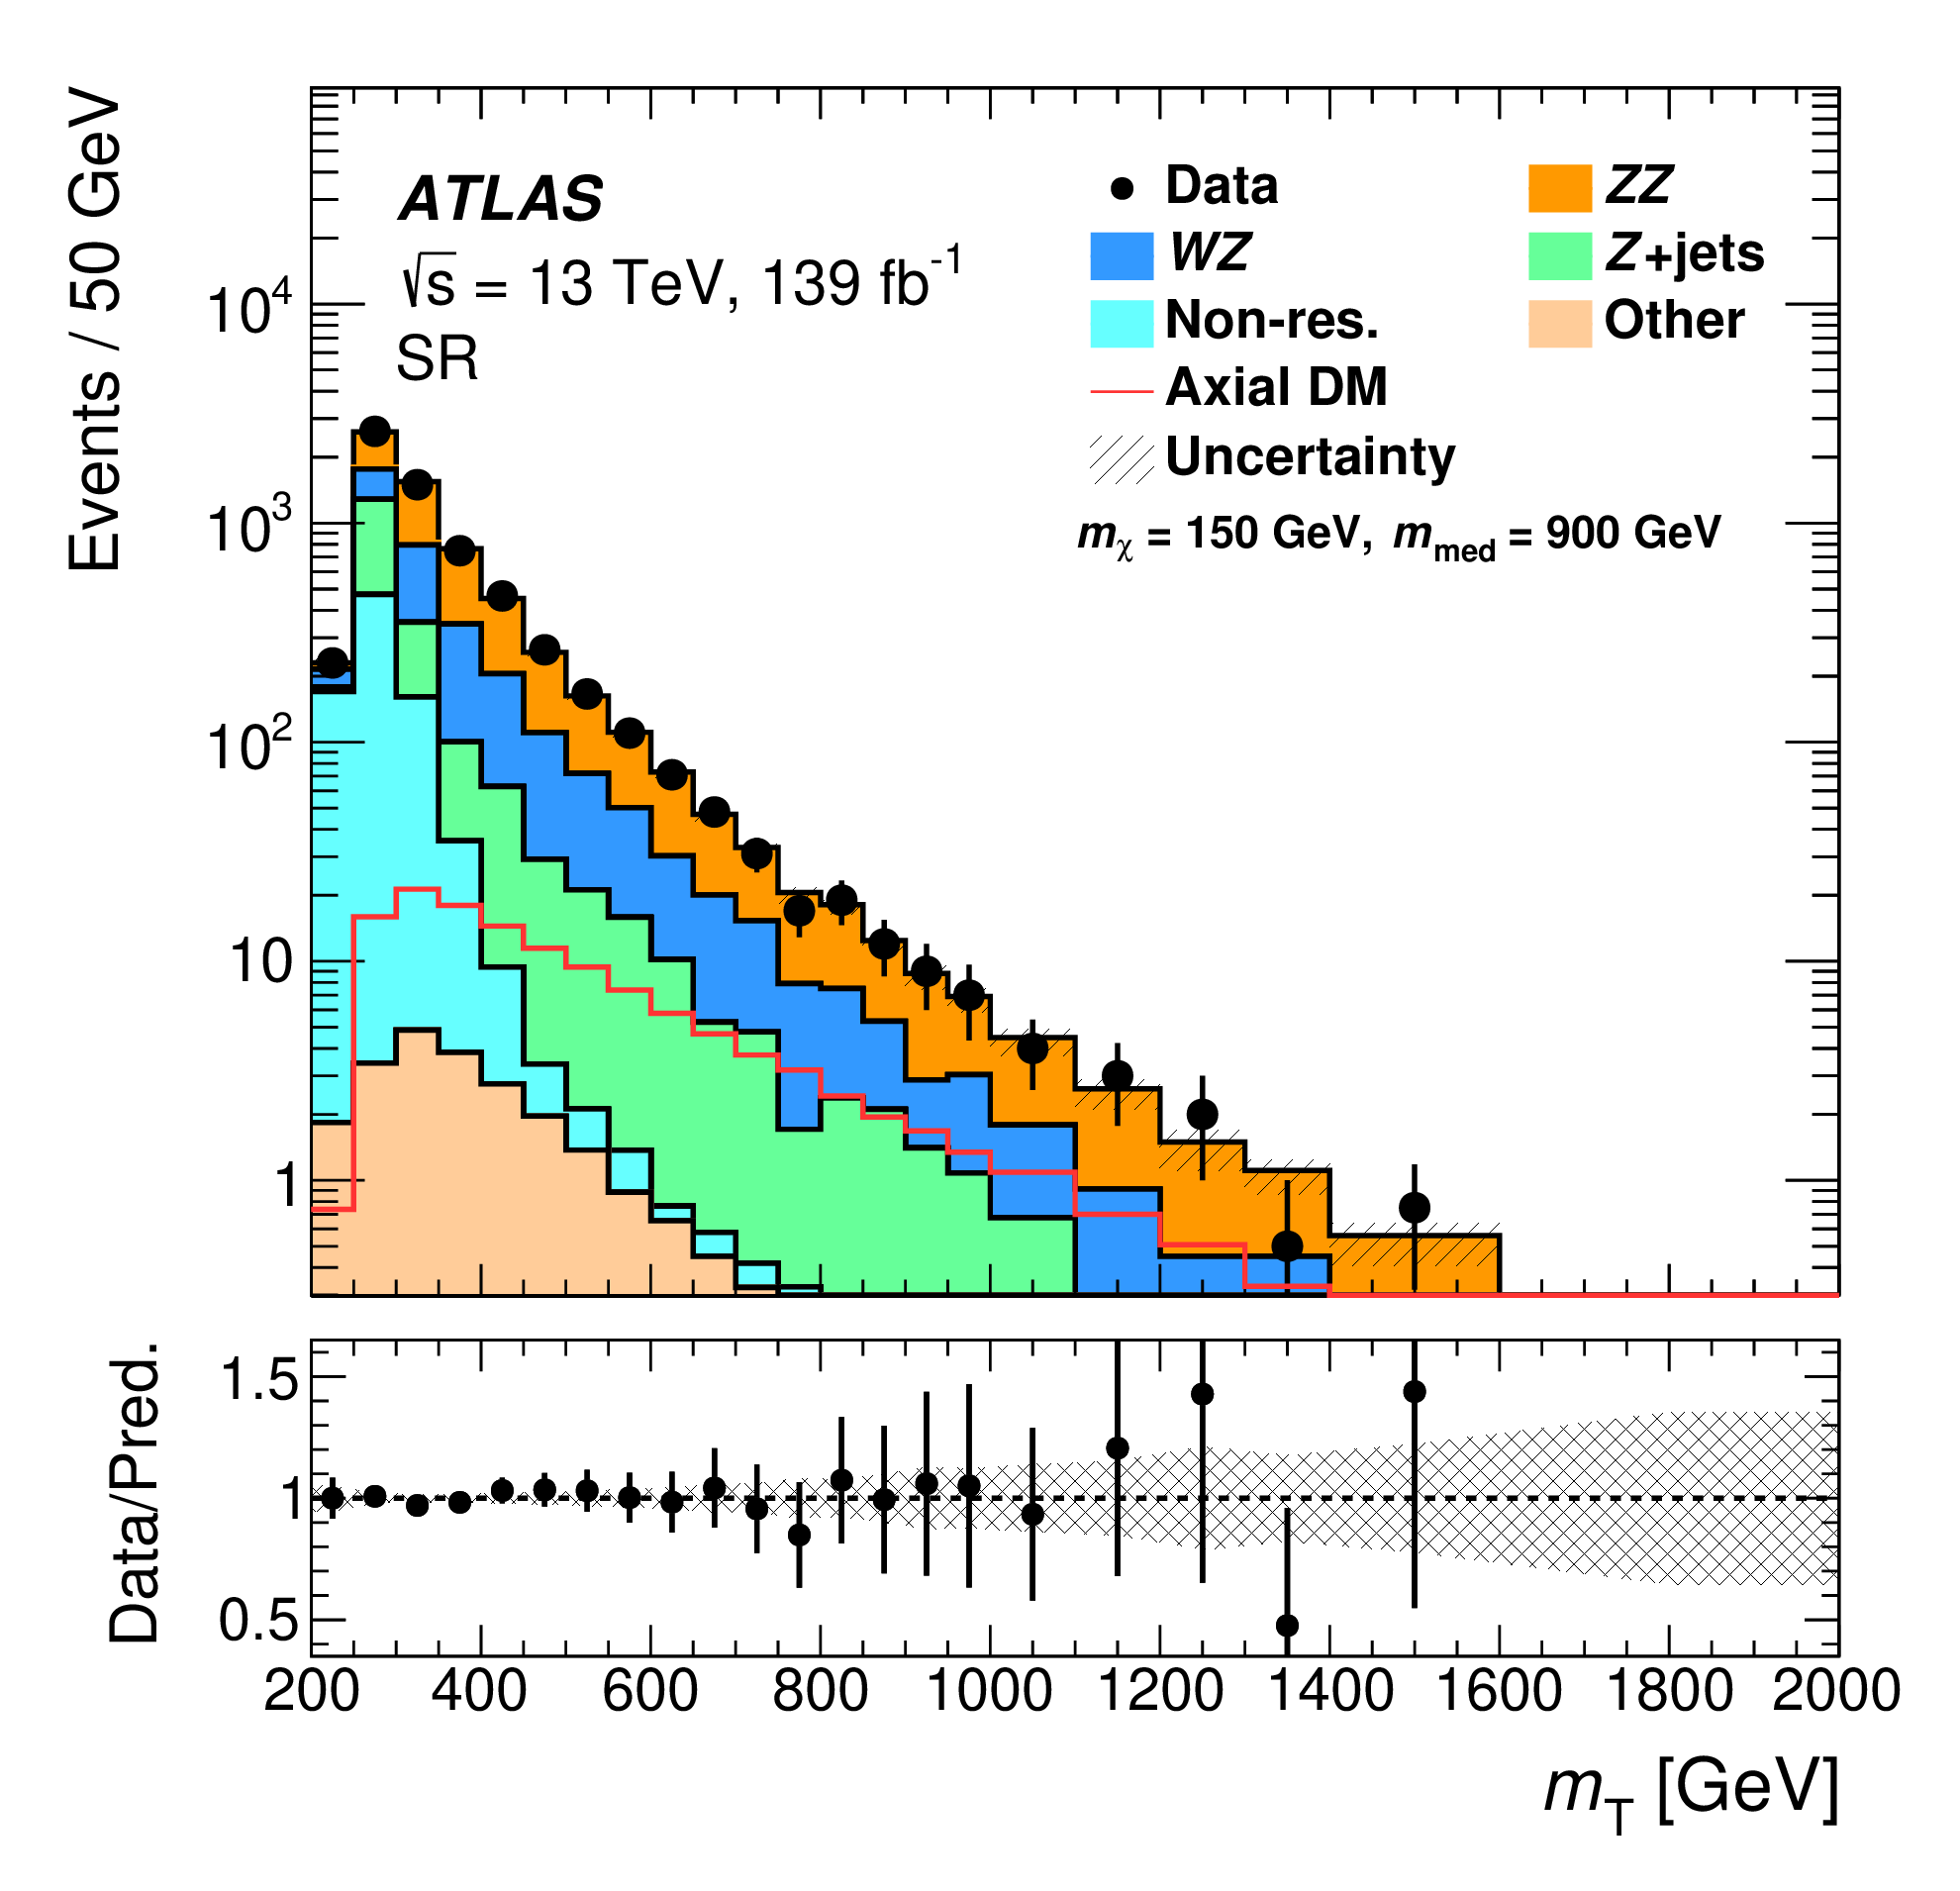
\includegraphics[width=0.4\linewidth]{figures/ch6-DM/fig_03b.png}}
    \hspace{0.5cm}
    \subfloat[]{
    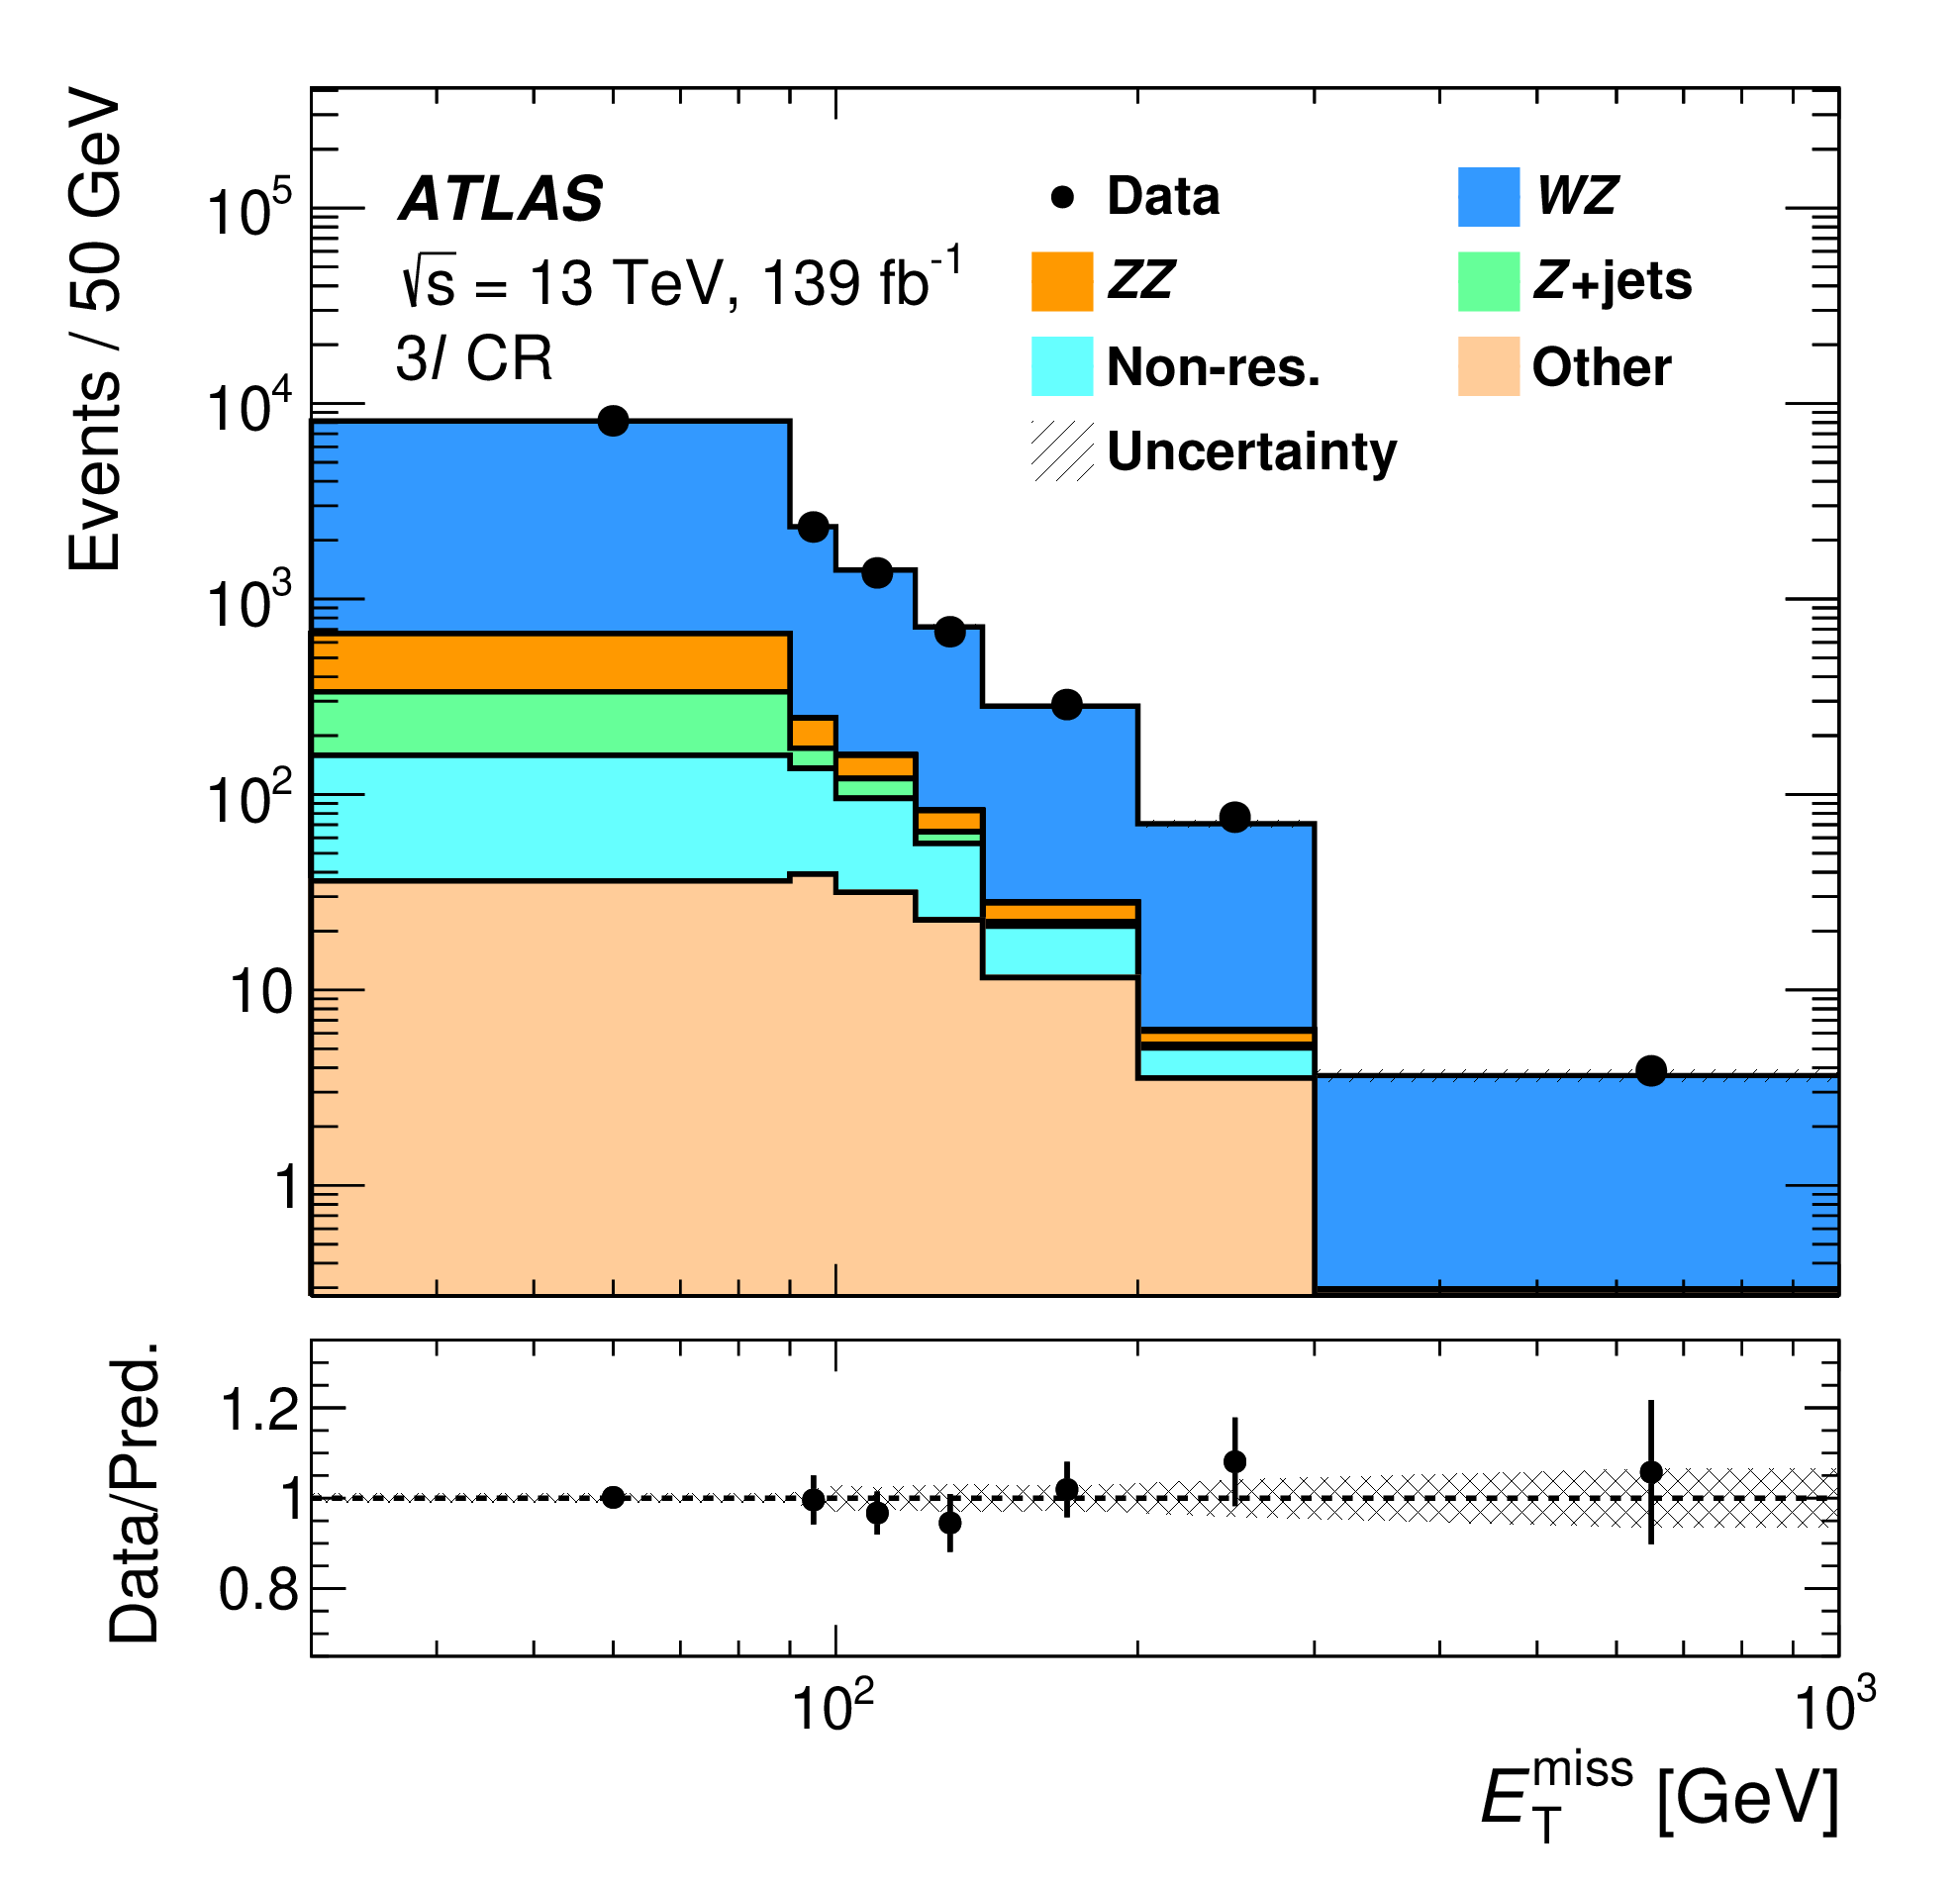
\includegraphics[width=0.4\linewidth]{figures/ch6-DM/fig_02a.png}} \\
    \subfloat[]{
    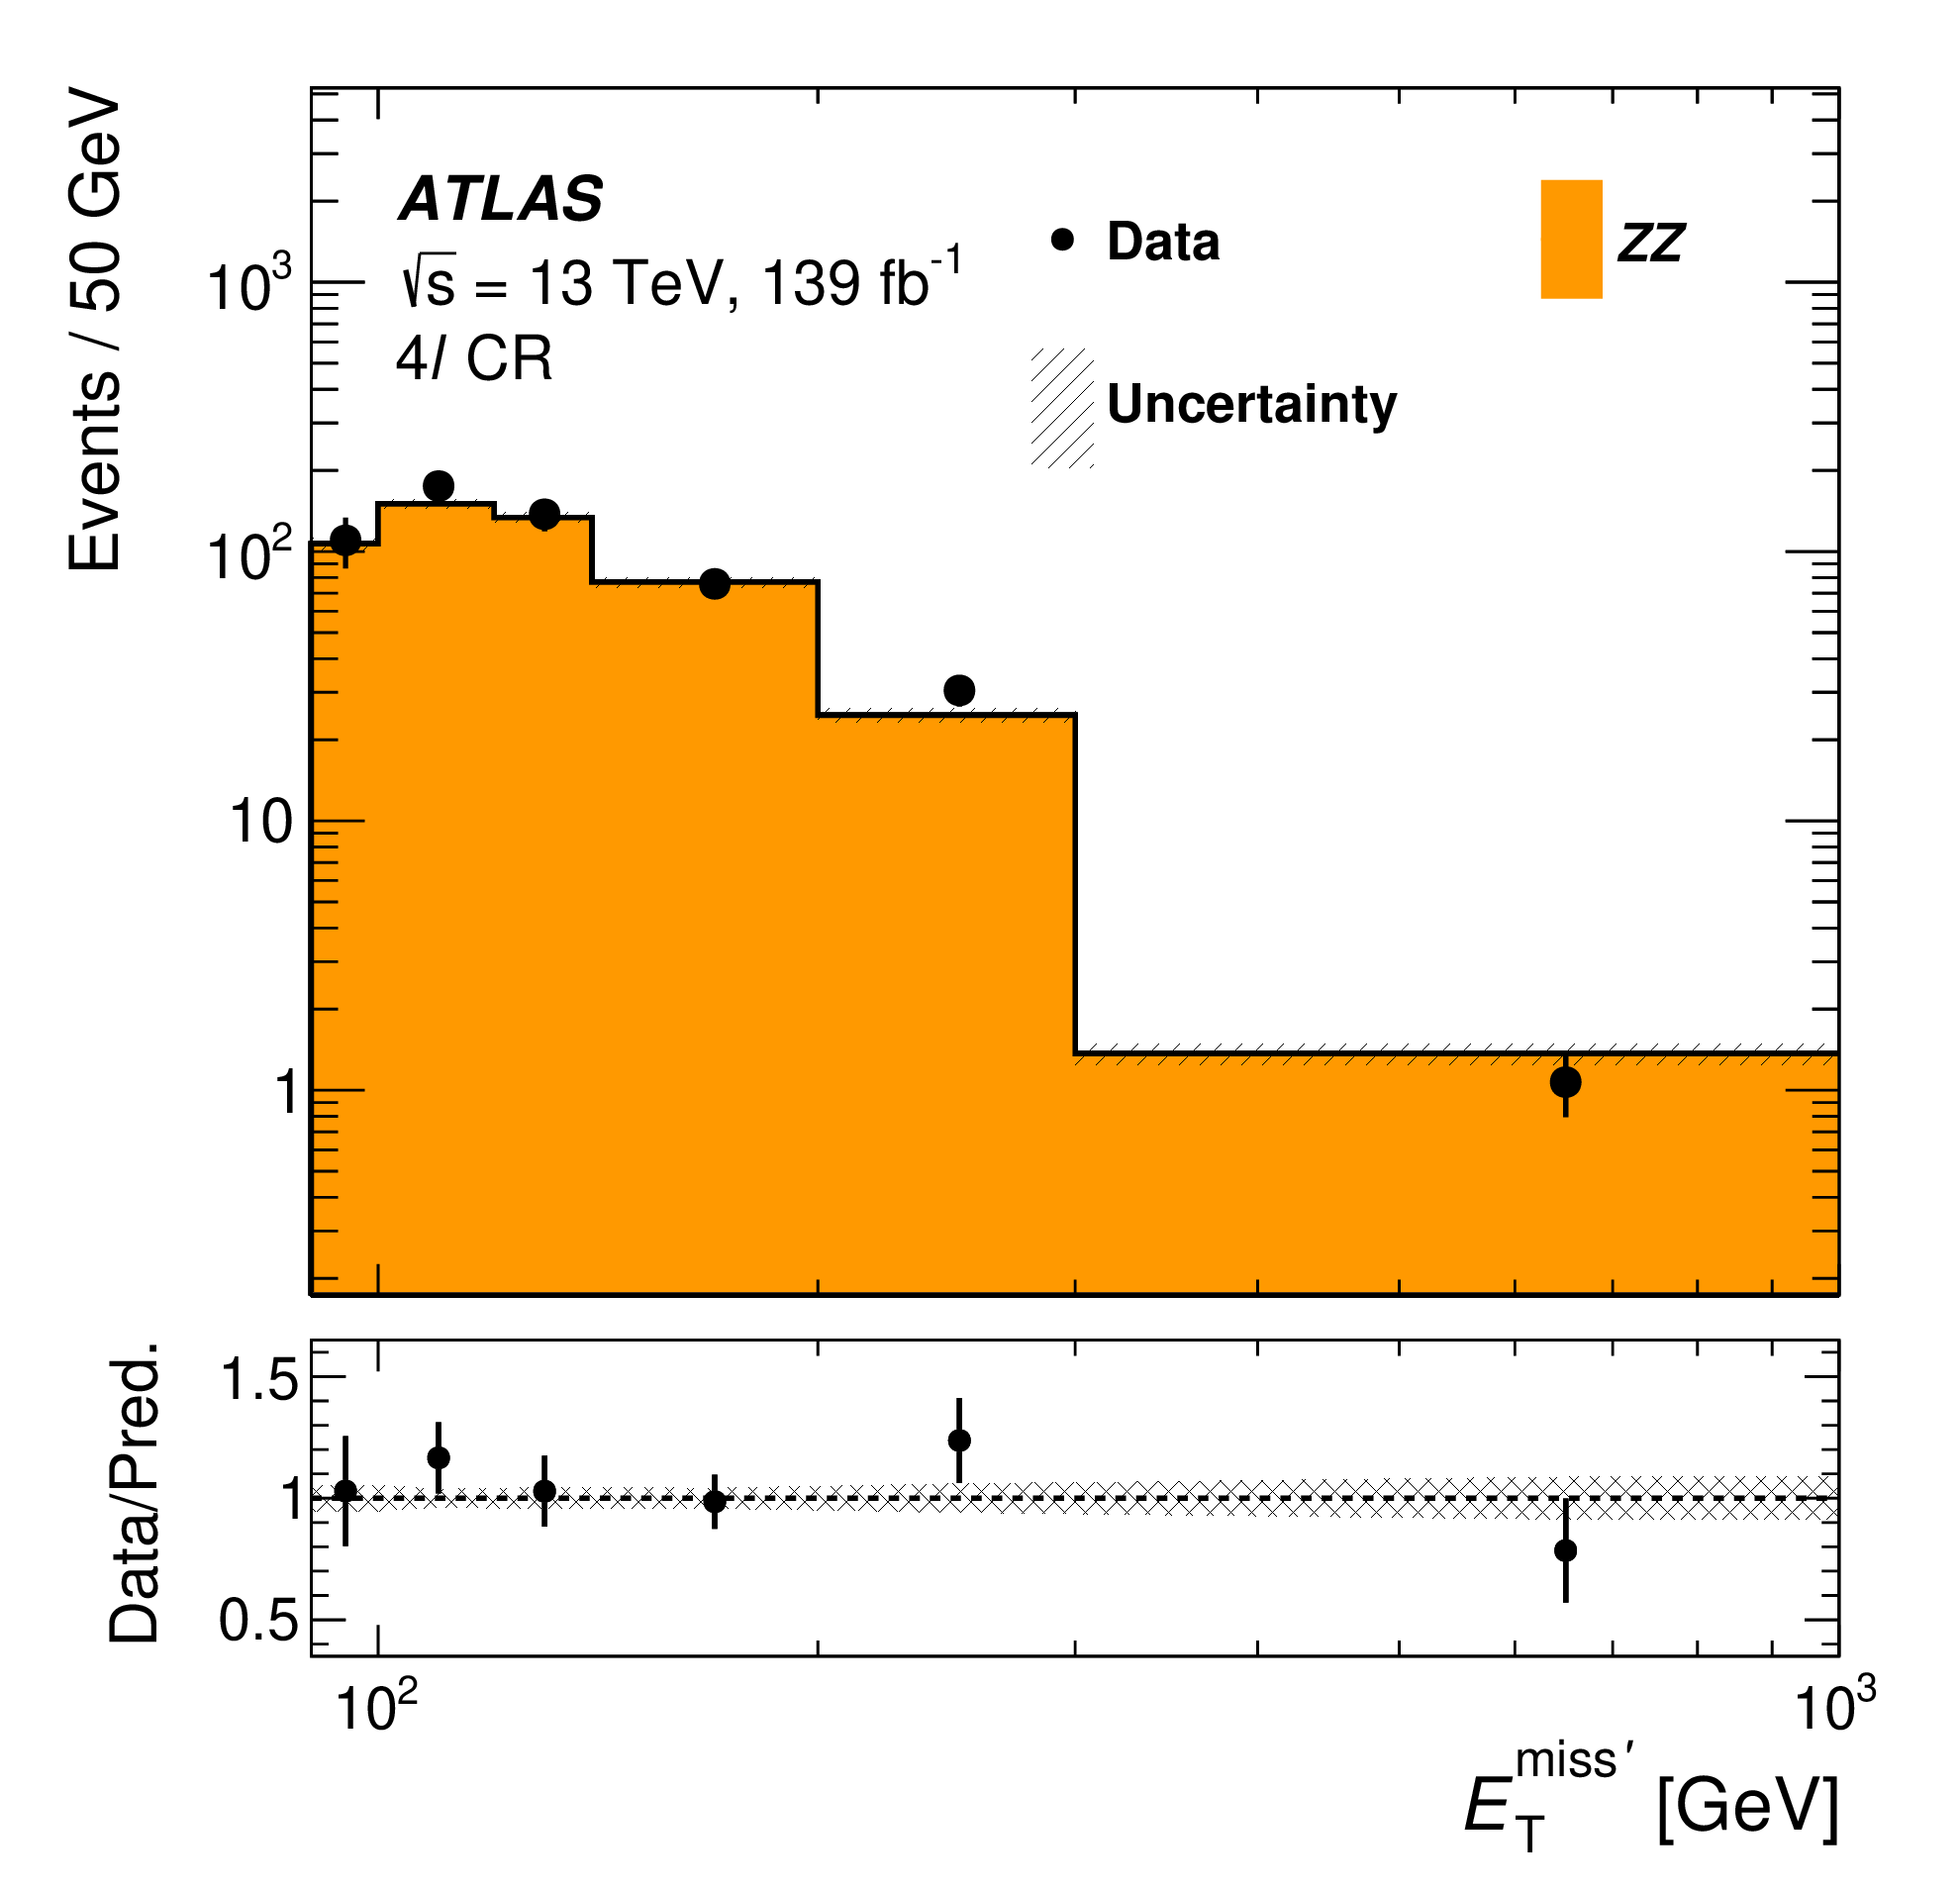
\includegraphics[width=0.4\linewidth]{figures/ch6-DM/fig_02b.png}}
    \hspace{0.5cm}
    \subfloat[]{
    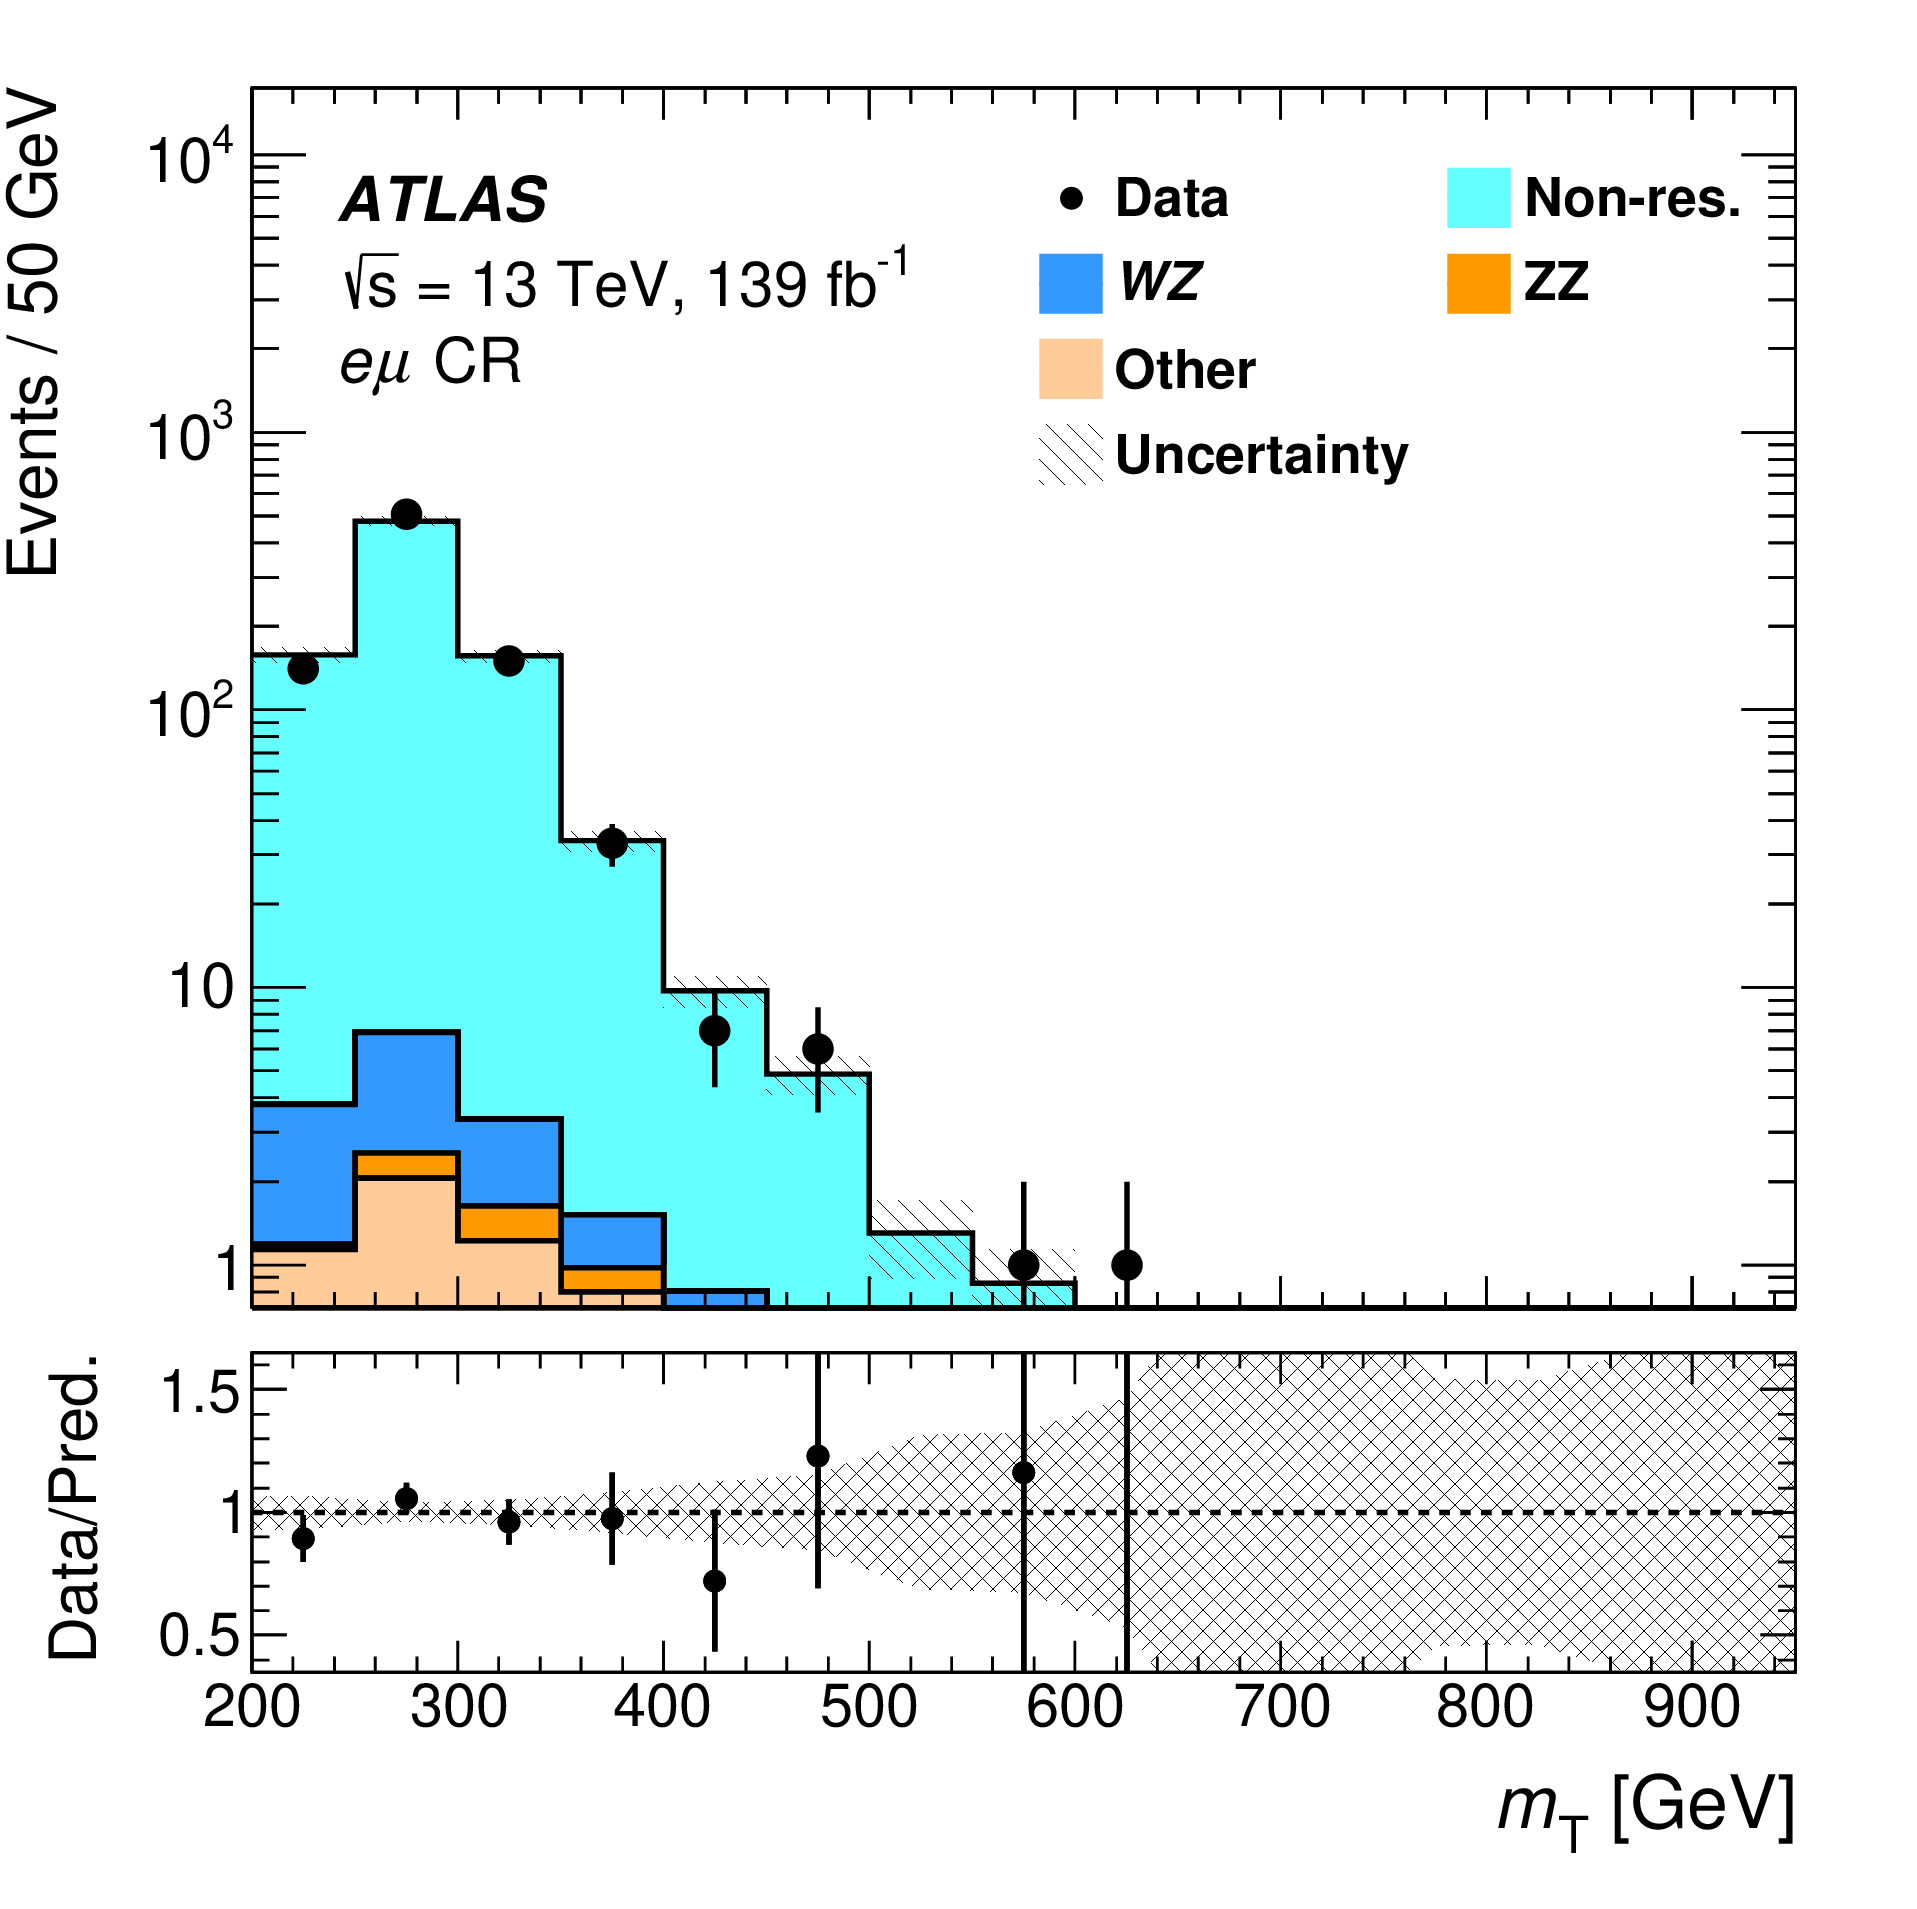
\includegraphics[width=0.4\linewidth]{figures/ch6-DM/fig_02d.png}}
    \caption{Data and MC prediction (post-fit) comparison in distributions: (a) $m_{\text{T}}^{\text{ZZ}}$ in SR (with Mono-$\text{Z}$ signal), (b) $E_{\text{T}}^{\text{miss}}$ in $3\ell$ CR, (c) $E_{\text{T}}^{\text{miss}}$ in $4\ell$ CR, and (d) $m_{\text{T}}^{\text{ZZ}}$ in $e\mu$ CR.}
    \label{fig:SR-CR-plot}
\end{figure}

%Example post-fit distributions in the CRs are shown in Figures~2(a)--2(c), after the simultaneous fit to the SR and CRs in the $ZH \to \ell\ell + \mathrm{inv}$ analysis. The data are well described by the fitted predictions, and the fit uses the same binning as shown in these figures.